% Options for packages loaded elsewhere
\PassOptionsToPackage{unicode}{hyperref}
\PassOptionsToPackage{hyphens}{url}
%
\documentclass[
]{book}
\usepackage{amsmath,amssymb}
\usepackage{iftex}
\ifPDFTeX
  \usepackage[T1]{fontenc}
  \usepackage[utf8]{inputenc}
  \usepackage{textcomp} % provide euro and other symbols
\else % if luatex or xetex
  \usepackage{unicode-math} % this also loads fontspec
  \defaultfontfeatures{Scale=MatchLowercase}
  \defaultfontfeatures[\rmfamily]{Ligatures=TeX,Scale=1}
\fi
\usepackage{lmodern}
\ifPDFTeX\else
  % xetex/luatex font selection
\fi
% Use upquote if available, for straight quotes in verbatim environments
\IfFileExists{upquote.sty}{\usepackage{upquote}}{}
\IfFileExists{microtype.sty}{% use microtype if available
  \usepackage[]{microtype}
  \UseMicrotypeSet[protrusion]{basicmath} % disable protrusion for tt fonts
}{}
\makeatletter
\@ifundefined{KOMAClassName}{% if non-KOMA class
  \IfFileExists{parskip.sty}{%
    \usepackage{parskip}
  }{% else
    \setlength{\parindent}{0pt}
    \setlength{\parskip}{6pt plus 2pt minus 1pt}}
}{% if KOMA class
  \KOMAoptions{parskip=half}}
\makeatother
\usepackage{xcolor}
\usepackage{longtable,booktabs,array}
\usepackage{calc} % for calculating minipage widths
% Correct order of tables after \paragraph or \subparagraph
\usepackage{etoolbox}
\makeatletter
\patchcmd\longtable{\par}{\if@noskipsec\mbox{}\fi\par}{}{}
\makeatother
% Allow footnotes in longtable head/foot
\IfFileExists{footnotehyper.sty}{\usepackage{footnotehyper}}{\usepackage{footnote}}
\makesavenoteenv{longtable}
\usepackage{graphicx}
\makeatletter
\def\maxwidth{\ifdim\Gin@nat@width>\linewidth\linewidth\else\Gin@nat@width\fi}
\def\maxheight{\ifdim\Gin@nat@height>\textheight\textheight\else\Gin@nat@height\fi}
\makeatother
% Scale images if necessary, so that they will not overflow the page
% margins by default, and it is still possible to overwrite the defaults
% using explicit options in \includegraphics[width, height, ...]{}
\setkeys{Gin}{width=\maxwidth,height=\maxheight,keepaspectratio}
% Set default figure placement to htbp
\makeatletter
\def\fps@figure{htbp}
\makeatother
\setlength{\emergencystretch}{3em} % prevent overfull lines
\providecommand{\tightlist}{%
  \setlength{\itemsep}{0pt}\setlength{\parskip}{0pt}}
\setcounter{secnumdepth}{5}
\usepackage{booktabs}
\ifLuaTeX
  \usepackage{selnolig}  % disable illegal ligatures
\fi
\usepackage[]{natbib}
\bibliographystyle{plainnat}
\usepackage{bookmark}
\IfFileExists{xurl.sty}{\usepackage{xurl}}{} % add URL line breaks if available
\urlstyle{same}
\hypersetup{
  pdftitle={Stocastic},
  pdfauthor={Ashan Jayamal},
  hidelinks,
  pdfcreator={LaTeX via pandoc}}

\title{Stocastic}
\author{Ashan Jayamal}
\date{2024-08-02}

\usepackage{amsthm}
\newtheorem{theorem}{Theorem}[chapter]
\newtheorem{lemma}{Lemma}[chapter]
\newtheorem{corollary}{Corollary}[chapter]
\newtheorem{proposition}{Proposition}[chapter]
\newtheorem{conjecture}{Conjecture}[chapter]
\theoremstyle{definition}
\newtheorem{definition}{Definition}[chapter]
\theoremstyle{definition}
\newtheorem{example}{Example}[chapter]
\theoremstyle{definition}
\newtheorem{exercise}{Exercise}[chapter]
\theoremstyle{definition}
\newtheorem{hypothesis}{Hypothesis}[chapter]
\theoremstyle{remark}
\newtheorem*{remark}{Remark}
\newtheorem*{solution}{Solution}
\begin{document}
\maketitle

{
\setcounter{tocdepth}{1}
\tableofcontents
}
\chapter{Premilaries}\label{premilaries}

\begin{definition}
\protect\hypertarget{def:unnamed-chunk-1}{}\label{def:unnamed-chunk-1}

Consider a set \(X\).
An \(\sigma\)-algebra \(\mathcal{F}\) of subsets of \(X\) is a collection \(\mathcal{F}\) of subsets of \(X\) satisfying the following conditions:

\begin{itemize}
\tightlist
\item
  \(\emptyset \in \mathcal{F}\)
\item
  If \(B \in \mathcal{F}\), then its complement \(B^c\) is also in \(F\)
\item
  If \(B_1, B_2, \ldots\) is a countable collection of sets in \(\mathcal{F}\), then their union \(\bigcup_{n=1}^\infty B_n\) is also in \(\mathcal{F}\).
\end{itemize}

\end{definition}

\section{Brownian Motion}\label{brownian-motion}

Let \((\Omega, F, P)\) be a probability space. A stochastic process is a measurable function \(X(t, \omega)\) defined on the product space \([0,\infty) \times \Omega\). In particular:

\begin{itemize}
\tightlist
\item
  For each \(t\), \(X(t, \cdot)\) is a random variable.
\item
  For each \(\omega\), \(X(\cdot, \omega)\) is a measurable function (called a sample path).
\end{itemize}

For convenience, the random variable \(X(t, \cdot)\) will be written as \(X(t)\) or \(X_t\).
Thus, a stochastic process \(X(t, \omega)\) can also be expressed as \(X(t)(\omega)\) or simply as \(X(t)\) or \(X_t\).

\section{Definition of Brownian Motion}\label{definition-of-brownian-motion}

\begin{definition}
\protect\hypertarget{def:Brownian_Motaion}{}\label{def:Brownian_Motaion}

A stochastic process \(B(t, \omega)\) is called a Brownian motion if it satisfies the following conditions:

\begin{enumerate}
\def\labelenumi{\arabic{enumi}.}
\tightlist
\item
  \(P(\{\omega : B(0, \omega) = 0\}) = 1\).
\item
  For any \(0 \leq s < t\), the random variable \(B(t) - B(s)\) is normally distributed with mean 0 and variance \(t - s\), i.e., for any \(a < b\),
  \[
  P(a \leq B(t) - B(s) \leq b) = \frac{1}{\sqrt{2\pi(t - s)}} \int_a^b e^{-x^2/2(t - s)} \, dx.
  \]
\item
  \(B(t, \omega)\) has independent increments, i.e., for any \(0 \leq t_1 < t_2 < \ldots < t_n\), the random variables
  \[B(t_1), B(t_2) - B(t_1), \ldots, B(t_n) - B(t_{n-1})\]
  are independent.
\item
  Almost all sample paths of \(B(t, \omega)\) are continuous functions, i.e.,
  \[P(\{\omega : B(\cdot, \omega) \text{ is continuous}\}) = 1\].
\end{enumerate}

\end{definition}

\section{Simple Properties of Brownian Motion}\label{simple-properties-of-brownian-motion}

Let\(B(t)\) be a fixed Brownian motion. We give below some simple properties that follow directly from the definition of Brownian motion.

\begin{proposition}
\protect\hypertarget{prp:unnamed-chunk-2}{}\label{prp:unnamed-chunk-2}For any \(t > 0\), \(B(t)\) is normally distributed with mean 0 and variance \(t\). For any \(s, t \geq 0\), we have \(\mathbb{E}[B(s)B(t)] = \min\{s, t\}\).
\end{proposition}

\begin{remark}
Regarding Definition @ref(def:Brownian\_Motaion), it can be proved that condition (2) and E{[}B(s)B(t){]} = min\{s, t\} imply condition (3).
\end{remark}

\begin{proof}
By condition (1), we have \(B(t) = B(t)−B(0)\) and so the first assertion follows from condition (2). With out loss of generlity, assume that \(s<t\).
\[\mathbb{E}[B(s)B(t)] = \mathbb{E}[B(s)(B(t) - B(s)) + B(s)^2]= 0 + s = s\]
which is equal to \(\min\{s, t\}\).
\end{proof}

\begin{proposition}[Translation Invariance]
\protect\hypertarget{prp:unnamed-chunk-5}{}\label{prp:unnamed-chunk-5}For a fixed \(t_0 \geq 0\), the stochastic process \(B(t) = B(t + t_0) - B(t_0)\) is also a Brownian motion.
\end{proposition}

\begin{proposition}[Scaling invariance]
\protect\hypertarget{prp:unnamed-chunk-6}{}\label{prp:unnamed-chunk-6}For any real number \(\lambda > 0\), the stochastic process
\(B(t) = \frac{B(\lambda t)}{\sqrt{\lambda}}\)
is also a Brownian motion.
\end{proposition}

\section{Wiener Integral}\label{wiener-integral}

\chapter{Introduction}\label{introduction}

\section{Events and Probability}\label{events-and-probability}

\begin{definition}
\protect\hypertarget{def:unnamed-chunk-7}{}\label{def:unnamed-chunk-7}

Let \(\Omega\) be a non-empty set. A \textbf{\(\sigma\)-field} \(\mathcal{F}\) on \(\Omega\) is a family of subsets of \(\Omega\) such that:

\begin{itemize}
\tightlist
\item
  The empty set \(\emptyset\) belongs to \(\mathcal{F}\);
\item
  If \(A\) belongs to \(\mathcal{F}\), then so does the complement \(\Omega \setminus A\);
\item
  If \(A_1, A_2, \ldots\) is a sequence of sets in \(\mathcal{F}\), then their union \(A_1 \cup A_2 \cup \cdots\) also belongs to \(\mathcal{F}\).
\end{itemize}

\end{definition}

\begin{example}
\protect\hypertarget{exm:unnamed-chunk-8}{}\label{exm:unnamed-chunk-8}a
\end{example}

\begin{definition}
\protect\hypertarget{def:unnamed-chunk-9}{}\label{def:unnamed-chunk-9}

Let \(\mathcal{F}\) be a \(\sigma\)-field on \(\Omega\). A probability measure \(P\) is a function
\(P : \mathcal{F} \to [0, 1]\)
such that

\begin{enumerate}
\def\labelenumi{\arabic{enumi}.}
\tightlist
\item
  \(P(\Omega) = 1\);
\item
  if \(A_1, A_2, \ldots\) are pairwise disjoint sets (that is, \(A_i \cap A_j = \emptyset\) for \(i \neq j\)) belonging to \(\mathcal{F}\), then
  \[
  P\left(\bigcup_{i=1}^{\infty} A_i\right) = \sum_{i=1}^{\infty} P(A_i);
  \]
\end{enumerate}

\begin{itemize}
\tightlist
\item
  The triple \((\Omega, \mathcal{F}, P)\) is called a probability space.
\item
  The sets belonging to \(\mathcal{F}\) are called events.
\item
  An event \(A\) is said to occur almost surely (a.s.) whenever \(P(A) = 1\).
\end{itemize}

\end{definition}

\begin{example}
\protect\hypertarget{exm:unnamed-chunk-10}{}\label{exm:unnamed-chunk-10}Let consider,

\begin{itemize}
\tightlist
\item
  \(\Omega=[0, 1]\) with the
\item
  \(\sigma\)-field =\(\mathcal{F} = \mathcal{B}([0, 1])\) of Borel sets \(B \subseteq [0, 1]\), and
\item
  Lebesgue measure \(P = \text{Leb}\) on \([0, 1]\).
\end{itemize}

Then \((\Omega, \mathcal{F}, P)\) is a probability space.

Recall that \(\text{Leb}\) is the unique measure defined on Borel sets such that
\[\text{Leb}[a, b] = b - a\]
for any interval \([a, b]\). (In fact, \(\text{Leb}\) can be extended to a larger \(\sigma\)-field, but we shall need Borel sets only.)
\end{example}

\begin{exercise}
\protect\hypertarget{exr:unnamed-chunk-11}{}\label{exr:unnamed-chunk-11}Show that if \(A_1, A_2, \ldots\) is an expanding sequence of events, that is
\[ A_1 \subseteq A_2 \subseteq A_3 \subseteq \cdots \]

then
\[ P\left(\bigcup_{n=1}^{\infty} A_n\right) = \lim_{n \to \infty} P(A_n). \]

Similarly, if \(A_1, A_2, \ldots\) is a contracting sequence of events, that is,
\[ A_1 \supseteq A_2 \supseteq A_3 \supseteq \cdots \]

then
\[ P\left(\bigcap_{n=1}^{\infty} A_n\right) = \lim_{n \to \infty} P(A_n). \]

\textbf{Hint:} Write \(A_1 \cup A_2 \cup \cdots\) as the union of a sequence of disjoint events: start with \(A_1\), then add a disjoint set to obtain \(A_1 \cup A_2\), then add a disjoint set again to obtain \(A_1 \cup A_2 \cup A_3\), and so on. Now that you have a sequence of disjoint sets, you can use the definition of a probability measure. To deal with the product \(A_1 \cap A_2 \cap \cdots\), write it as a union of some events with the aid of De Morgan's law.
\end{exercise}

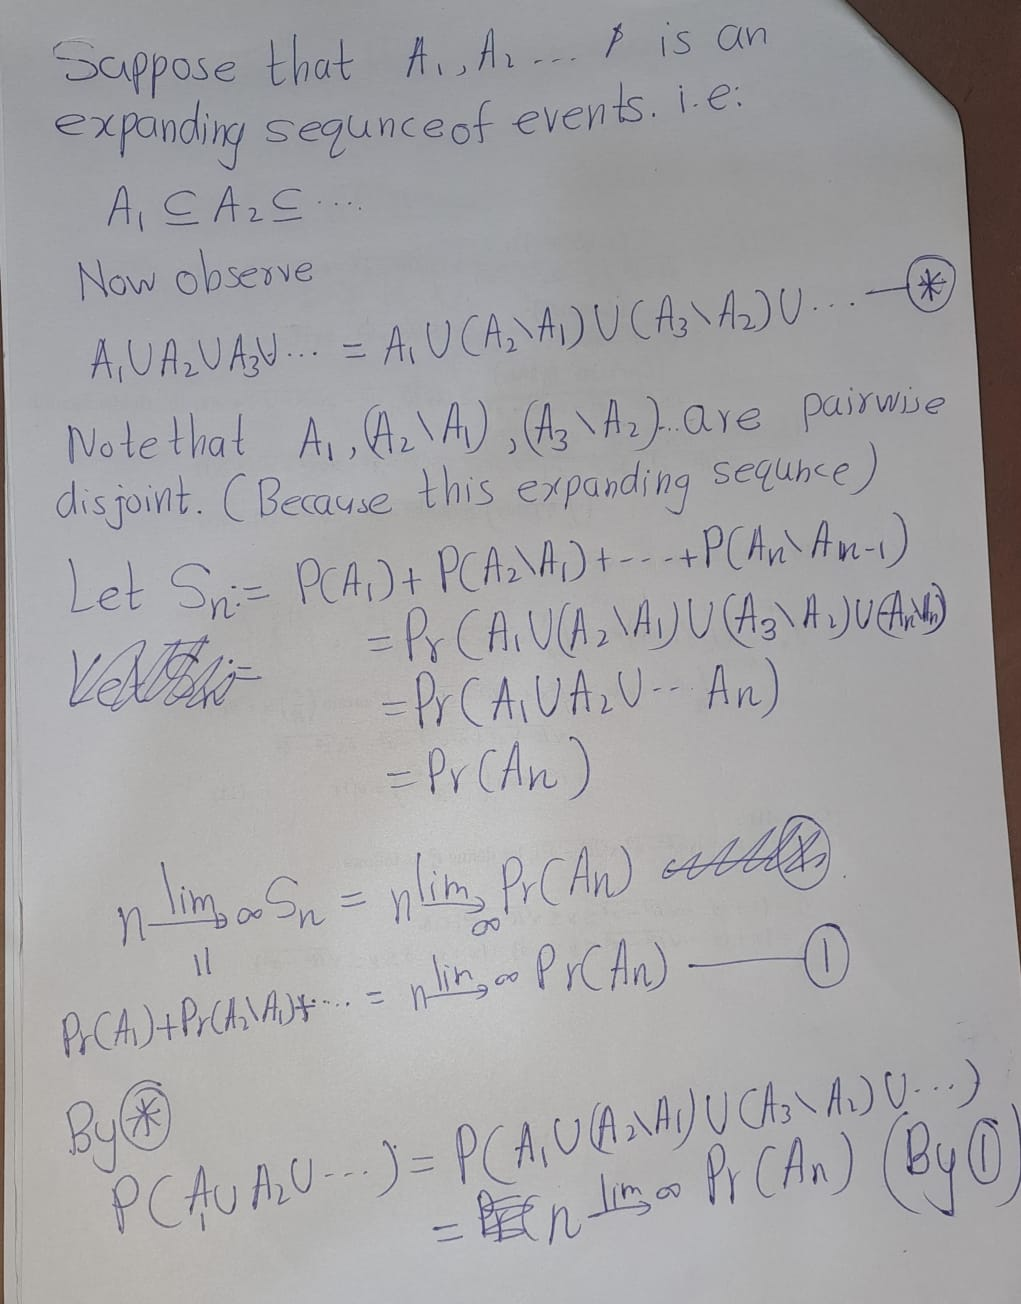
\includegraphics[width=18cm,height=\textheight]{fig/fig1.jpg}
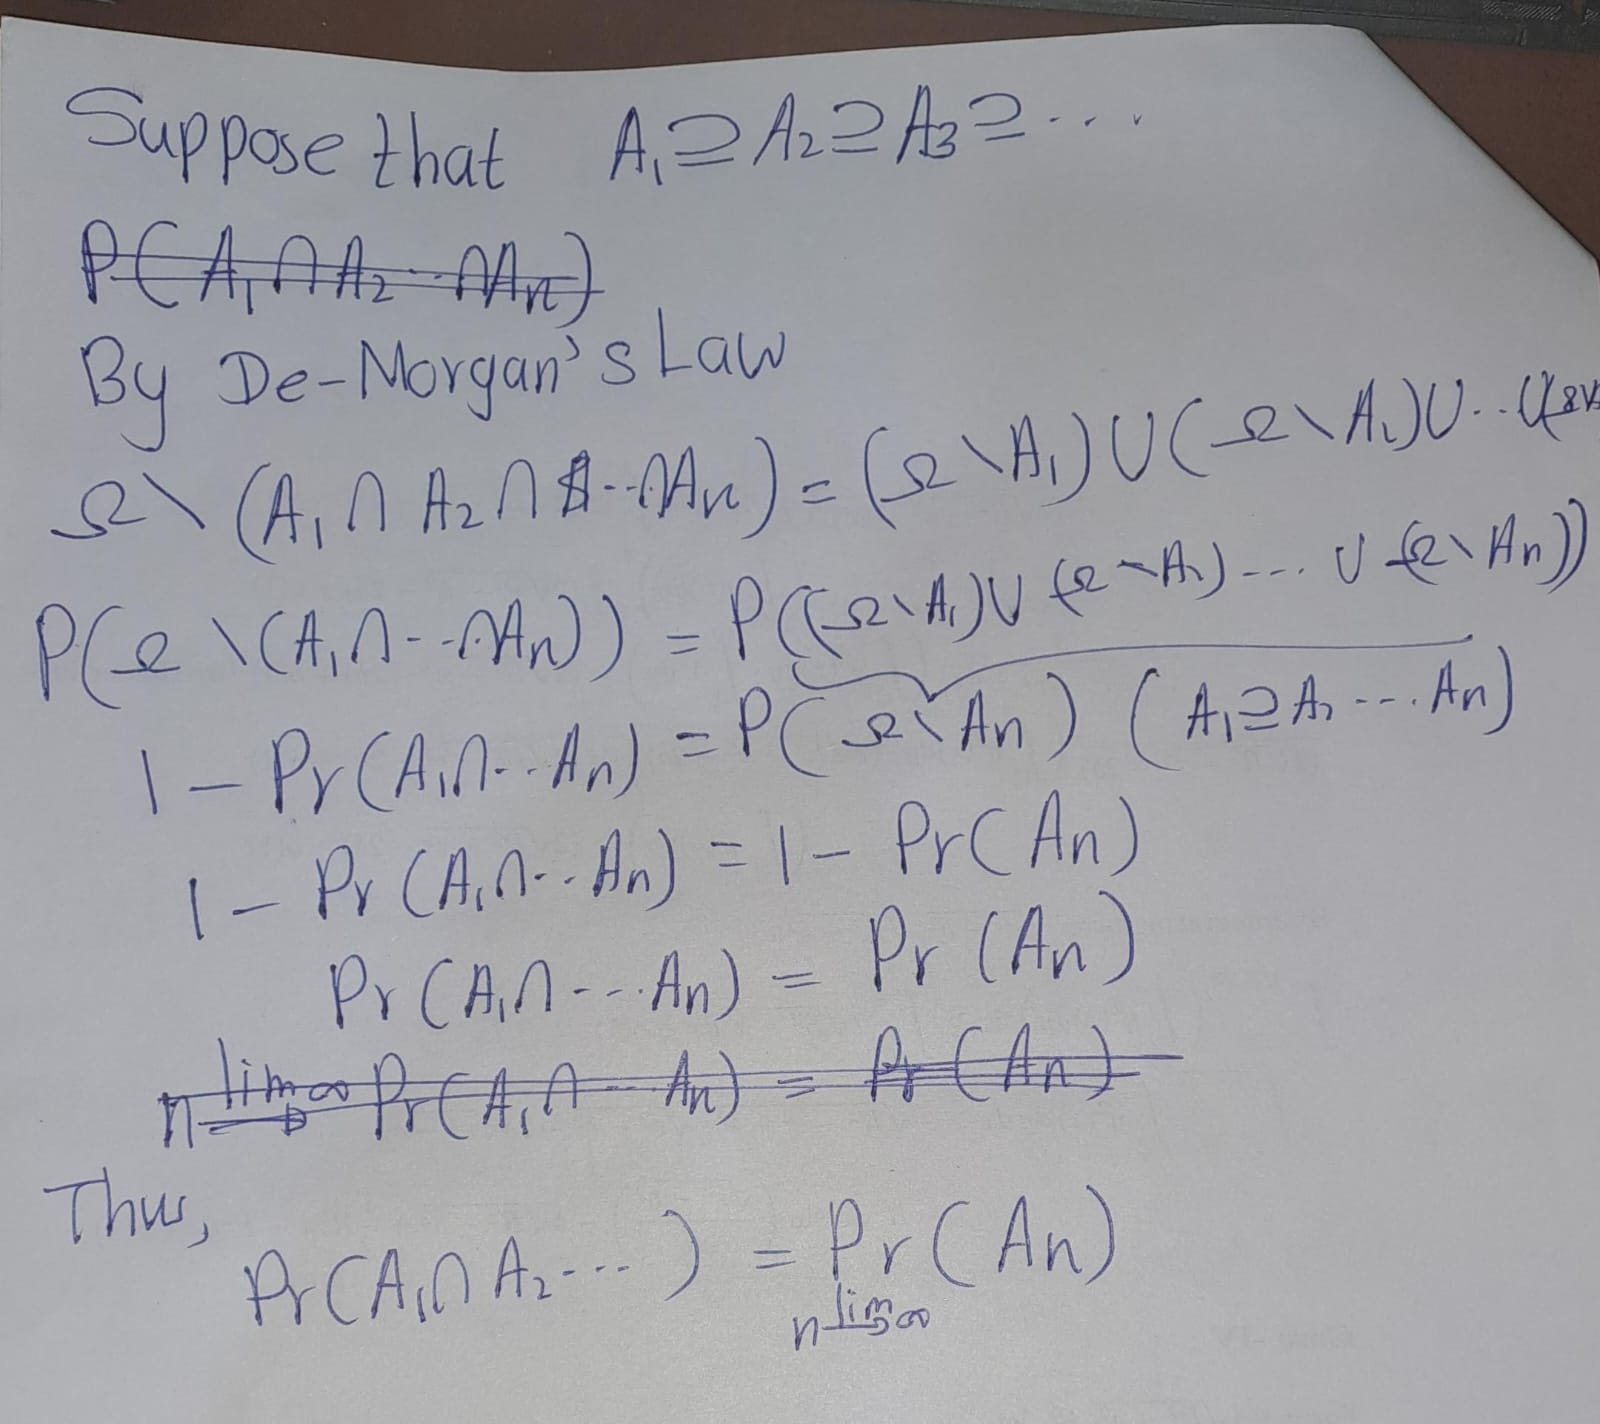
\includegraphics[width=18cm,height=\textheight]{fig/fig2.jpg}

\begin{lemma}[Borei-Cantelli]
\protect\hypertarget{lem:unnamed-chunk-12}{}\label{lem:unnamed-chunk-12}Let \(A_1, A_2, \ldots\) be a sequence of events such that \(P(A_1) + P(A_2) + \cdots < \infty\)
and let \(B_n = A_n \cup A_{n+1} \cup \cdots\). Then \(P(B_1 \cap B_2 \cap \cdots) = 0\).
\end{lemma}

\begin{exercise}
\protect\hypertarget{exr:unnamed-chunk-13}{}\label{exr:unnamed-chunk-13}Prove the Borel-Cantelli lemma above.

\textbf{Hint}: \(B_1, B_2, \ldots\) is a contracting sequence of events.
\end{exercise}

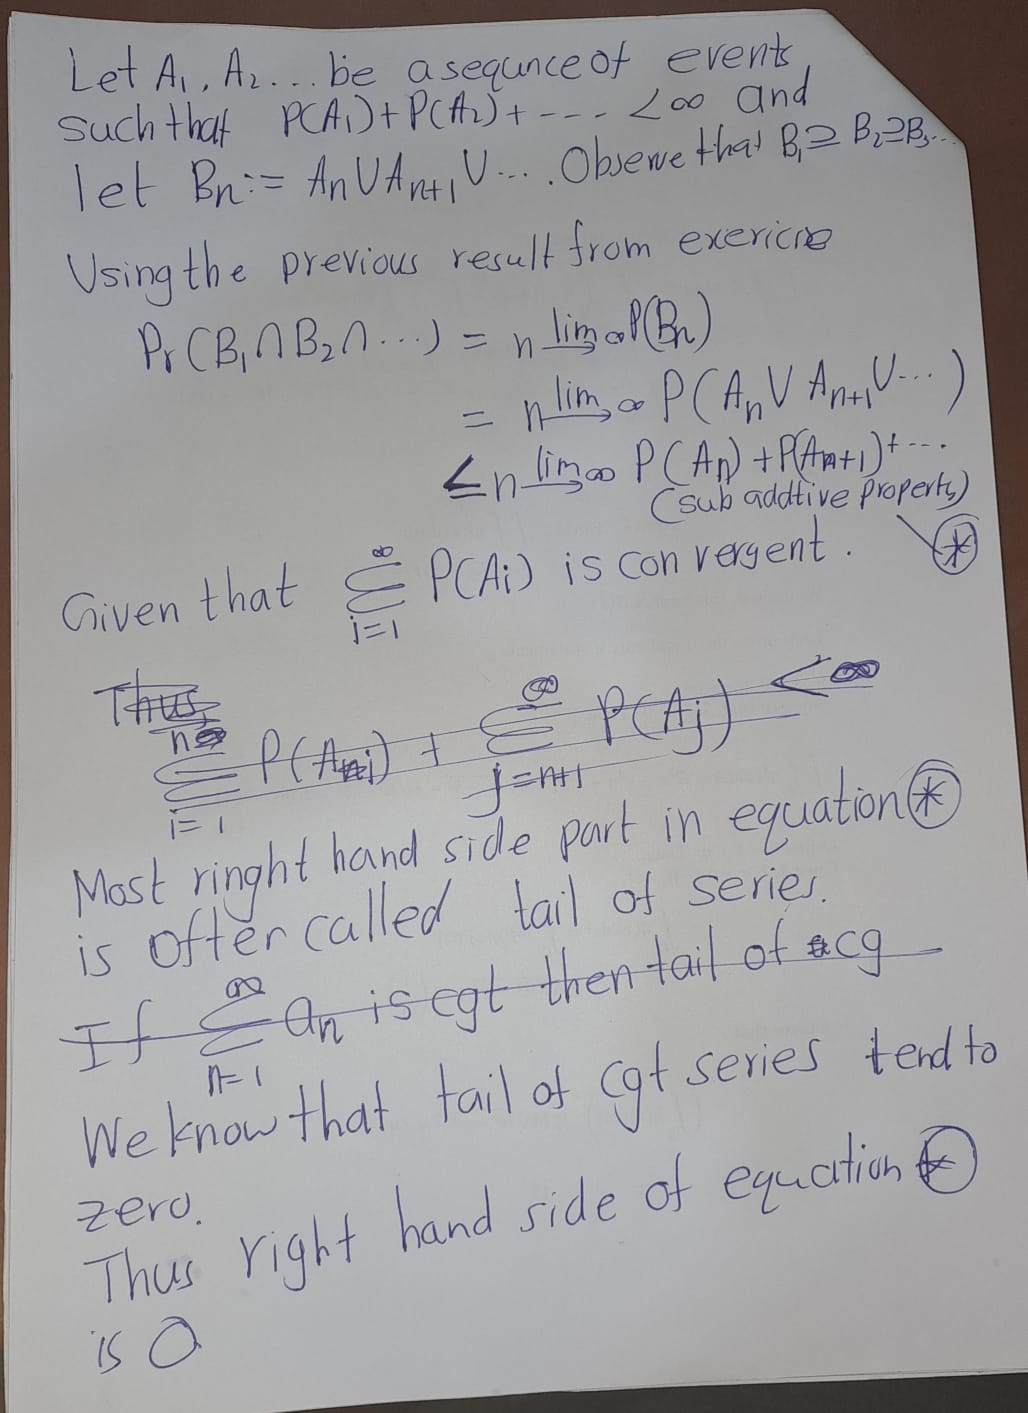
\includegraphics[width=18cm,height=\textheight]{fig/fig3.jpg}
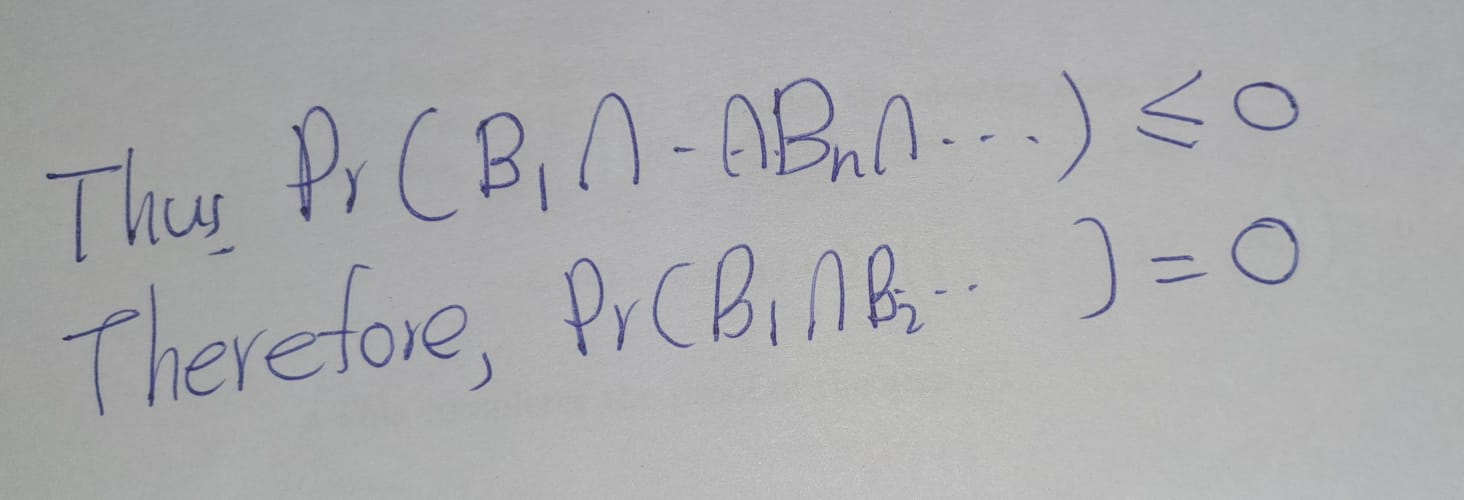
\includegraphics[width=18cm,height=\textheight]{fig/fig4.jpg}

\section{Random Variables}\label{random-variables}

\begin{definition}
\protect\hypertarget{def:unnamed-chunk-14}{}\label{def:unnamed-chunk-14}If \(\mathcal{F}\) is a \(\sigma\)-field on \(\Omega\), then a function \(X : \Omega \to \mathbb{R}\) is said to be \textbf{\(\mathcal{F}\)-measurable} if
\[\{\omega \in \Omega : X(\omega) \in B\}=X^{-1}(\omega)\]
for every Borel set \(B \in \mathcal{B}(\mathbb{R})\).\\
If \((\Omega, \mathcal{F}, P)\) is a probability space, then such a function \(X\) is called a \textbf{random variable.}
\end{definition}

\begin{definition}
\protect\hypertarget{def:unnamed-chunk-15}{}\label{def:unnamed-chunk-15}The \(\sigma\)-field \textbf{\(\sigma(X)\) generated by a random variable \(X : \Omega \to \mathbb{R}\)} consists of all sets
of the form \(\{\omega \in \Omega : X(\Omega)\in B\}\), where \(B\) is a Borel set in \(\mathbb{R}\).
\end{definition}

\begin{definition}
\protect\hypertarget{def:unnamed-chunk-16}{}\label{def:unnamed-chunk-16}The \(\sigma\)-field \(\sigma(\{X_i : i \in I\})\) generated by a family \(\{X_i : i \in I\}\) of random variables
is defined to be the smallest \(\sigma\)-field containing all events of the form \(\{X_i \in B\}\),
where \(B\) is a Borel set in \(\mathbb{R}\) and \(i \in I\).
\end{definition}

\begin{exercise}
\protect\hypertarget{exr:unnamed-chunk-17}{}\label{exr:unnamed-chunk-17}We call \(f : \mathbb{R} \to \mathbb{R}\) a \textbf{Borel function} if the inverse image \(f^{-1}(B)\) of any Borel set \(B\) in \(\mathbb{R}\) is a Borel set. Show that if \(f\) is a Borel function and \(X\) is a random variable, then the composition \(f(X)\) is \(\sigma(X)\)-measurable.

\emph{Hint}: Consider the event \(\{f(X) \in B\}\), where \(B\) is an arbitrary Borel set. Can this
event be written as \(\{X \in A\}\) for some Borel set \(A\)?
\end{exercise}

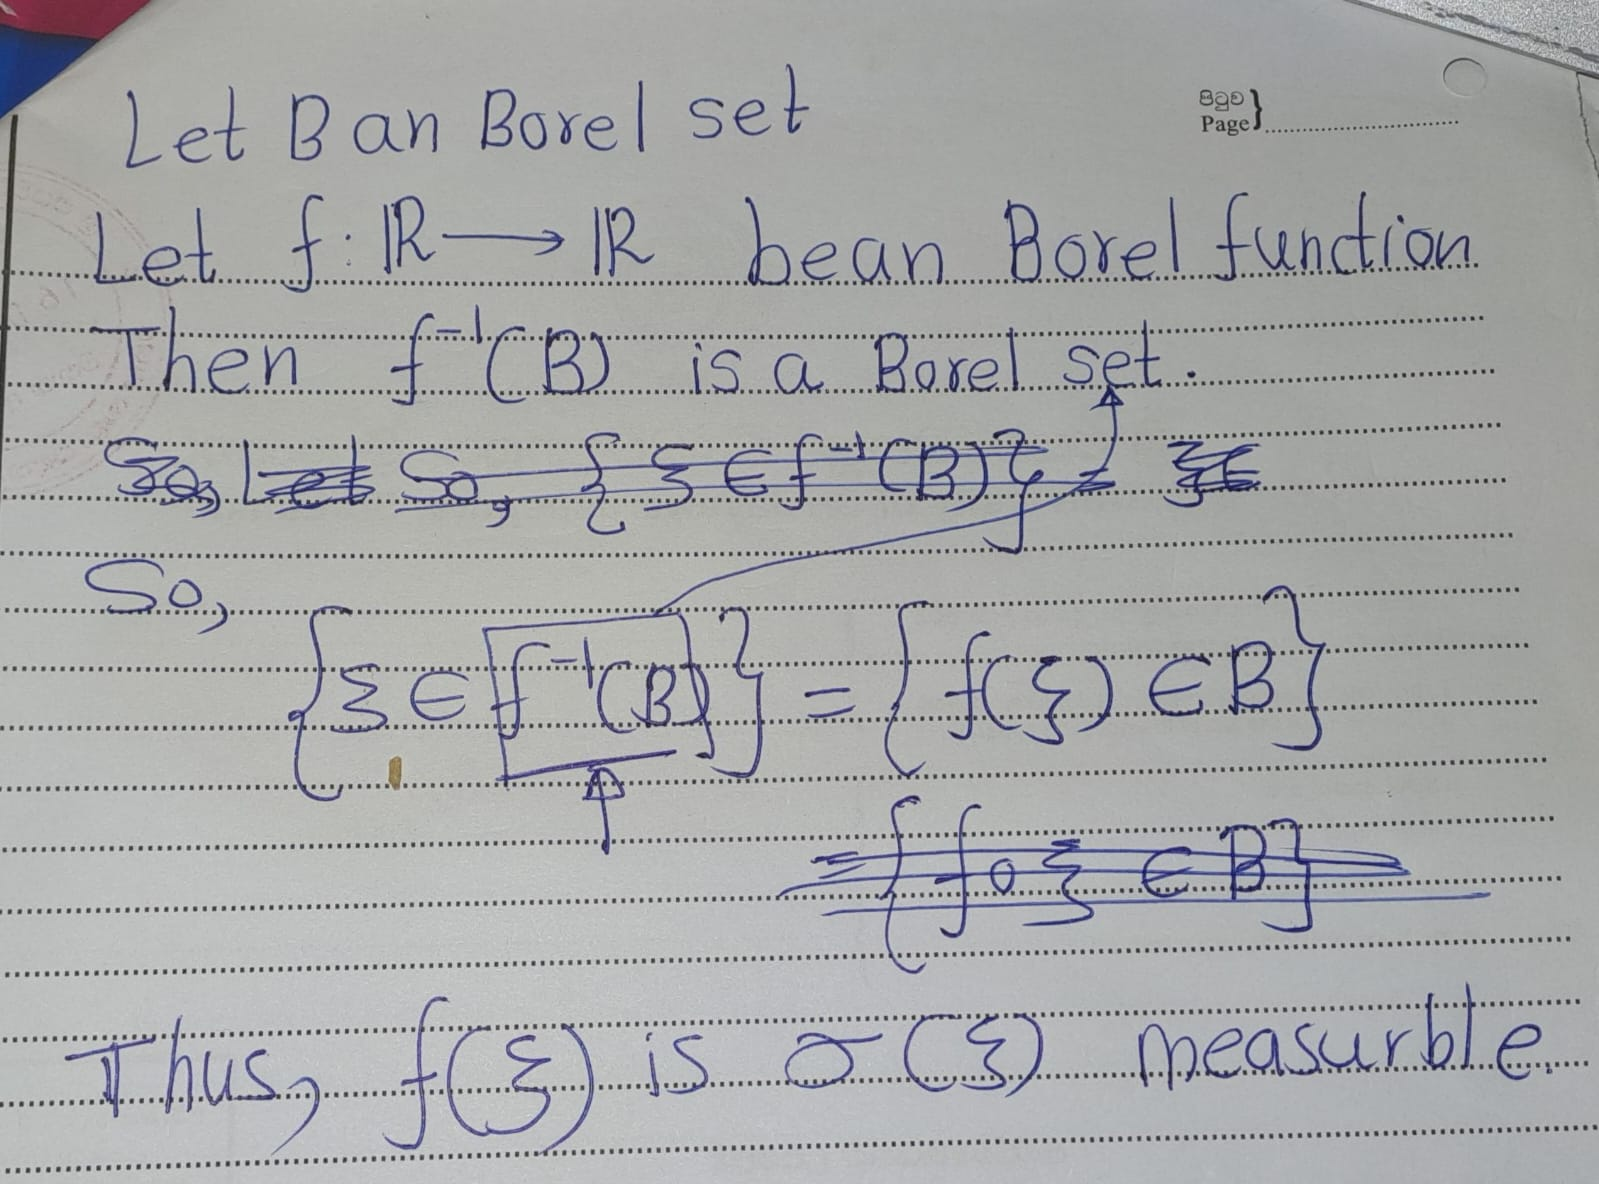
\includegraphics[width=18cm,height=\textheight]{fig/fig5.jpg}

\begin{lemma}[Doob-Dynkin]
\protect\hypertarget{lem:unnamed-chunk-18}{}\label{lem:unnamed-chunk-18}Let \(X\) be a random variable. Then each \(\sigma(X)\)-measurable random variable \(\eta\) can
be written as
\[
\eta = f(X)
\]
for some Borel function \(f : \mathbb{R} \to \mathbb{R}\).
\end{lemma}

\begin{proof}
Omiited
\end{proof}

\begin{definition}
\protect\hypertarget{def:unnamed-chunk-20}{}\label{def:unnamed-chunk-20}Every random variable \(X : \Omega \to \mathbb{R}\) gives rise to a probability measure
\[ P_X(B) = P\{X \in B\} \]
on \(\mathbb{R}\) defined on the \(\sigma\)-field of Borel sets \(B \in \mathcal{B}(\mathbb{R})\). We call \(P_X\) the distribution
of \(X\). The function \(F_X : \mathbb{R} \to [0, 1]\) defined by
\[ F_X(x) = P\{X \leq x\} \]
is called the cumulative distribution function (CDF) of \(X\).
\end{definition}

\begin{exercise}
\protect\hypertarget{exr:unnamed-chunk-21}{}\label{exr:unnamed-chunk-21}Show that the distribution function \(F\) is non-decreasing, right-continuous, and
\[
\lim_{x \to -\infty} F_{\xi}(x) = 0, \quad \lim_{x \to +\infty} F_{\Xi}(x) = 1.
\]

\textbf{Hint:} For example, to verify right-continuity show that \(F_{\xi}(x_n) \to F_{\xi}(x)\) for any decreasing sequence \(x_n\) such that \(x_n \to x\). You may find the results of Exercises useful.
\end{exercise}

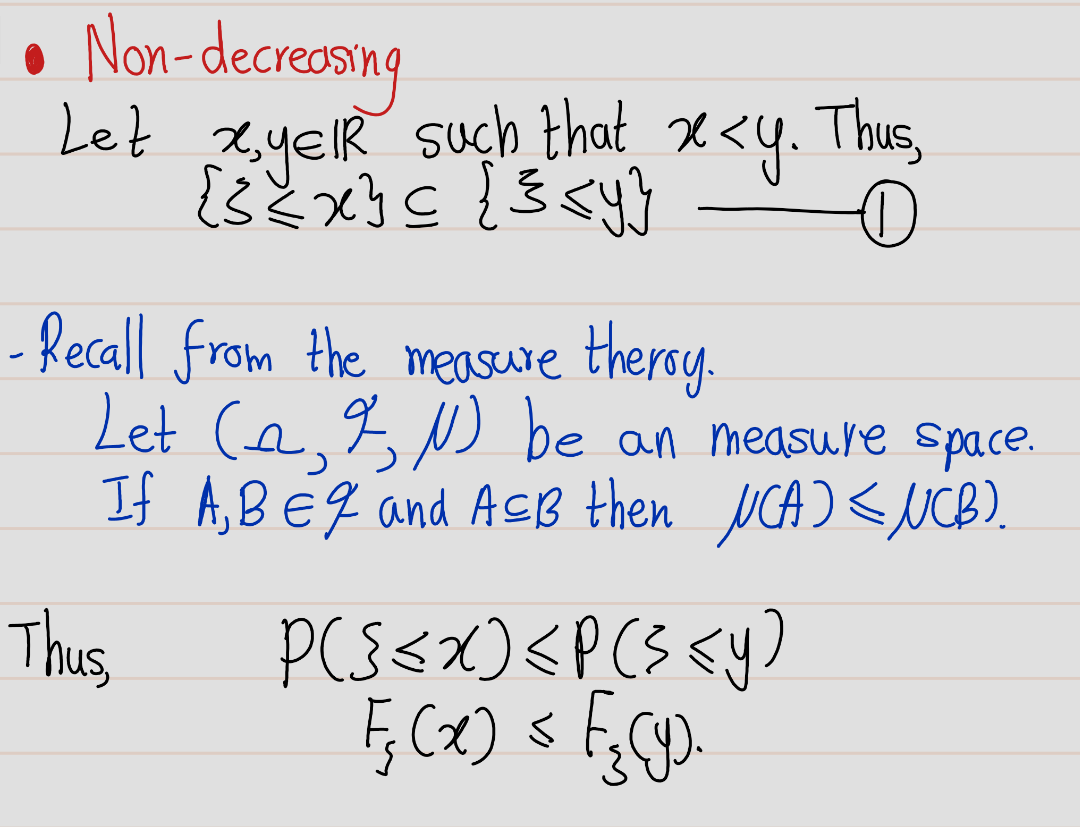
\includegraphics[width=18cm,height=\textheight]{fig/fig ex1.4-1.png}
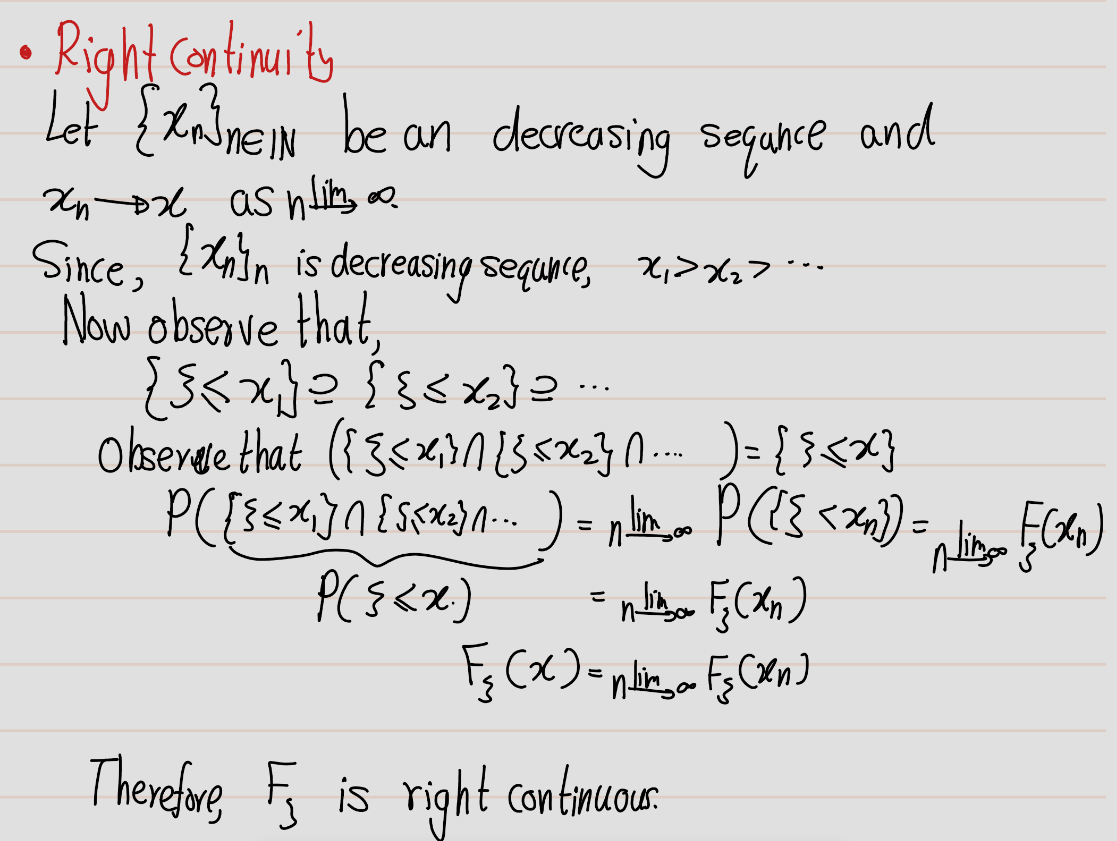
\includegraphics[width=18cm,height=\textheight]{fig/fig ex1.4-2.png}
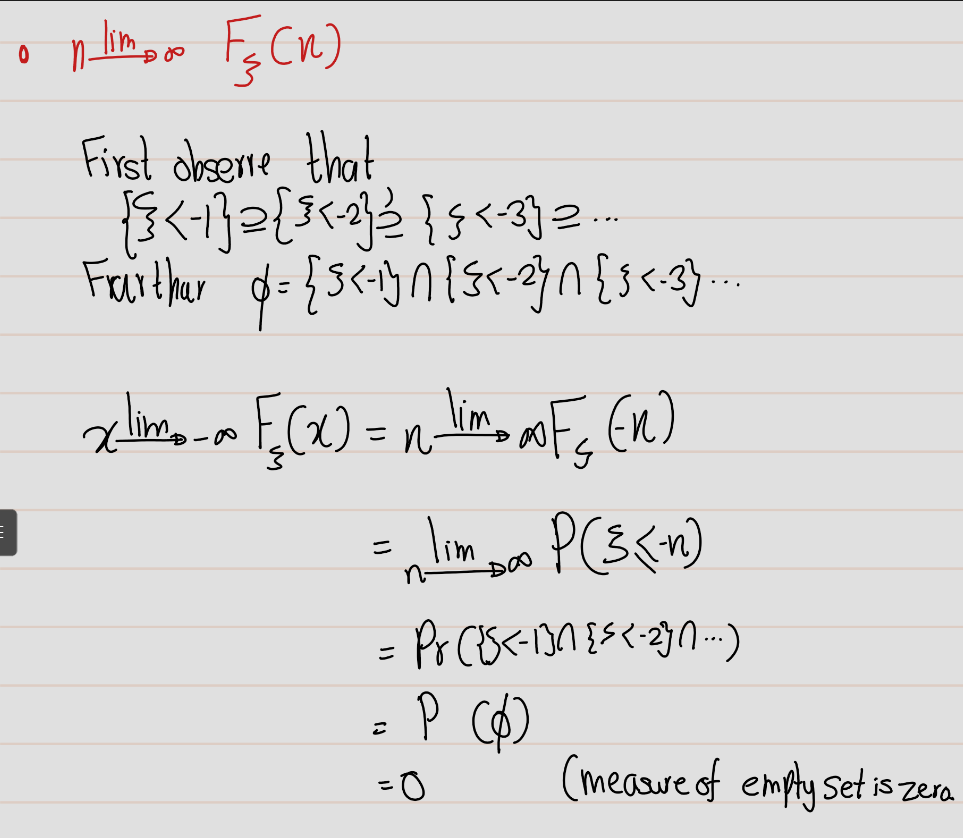
\includegraphics[width=18cm,height=\textheight]{fig/fig ex1.4-3.png}
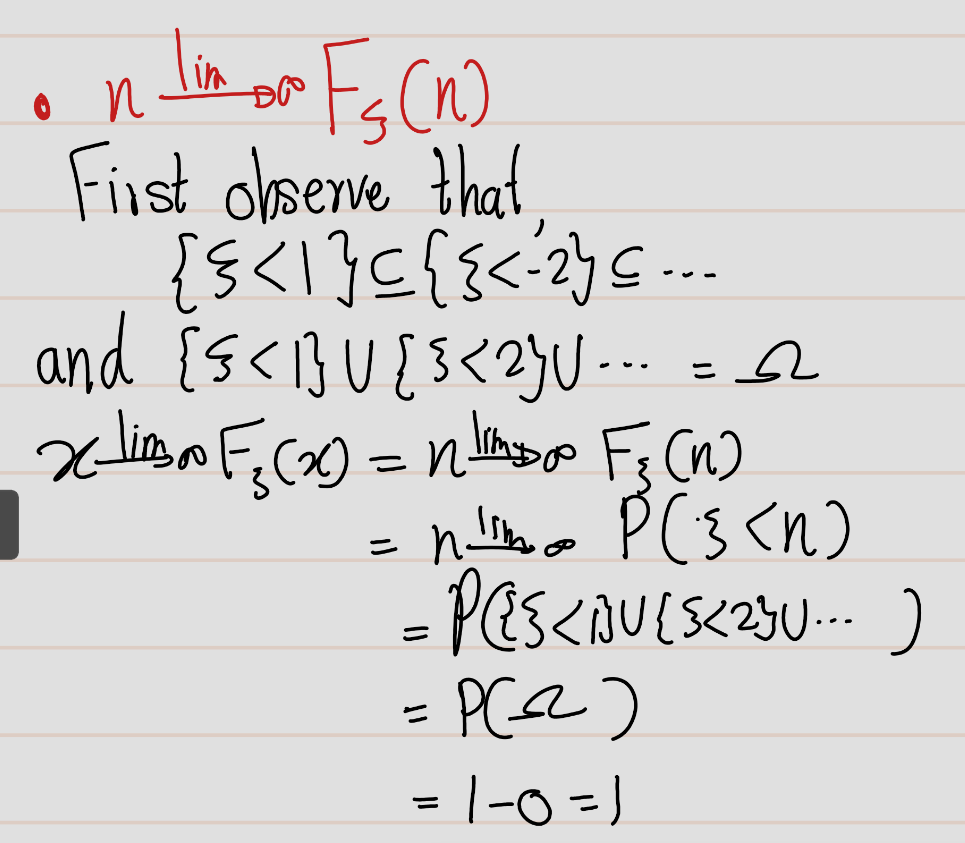
\includegraphics[width=18cm,height=\textheight]{fig/fig ex1.4-4.png}

\begin{definition}
\protect\hypertarget{def:unnamed-chunk-22}{}\label{def:unnamed-chunk-22}If there is a Borel function \(f: \mathbb{R} \to \mathbb{R}\) such that for any Borel set \(B \subset \mathbb{R}\)
\[
P\{\xi \in B\} = \int_B f_\xi(x) \, dx,
\]
then \(\xi\) is said to be a random variable with absolutely continuous distribution and \(f_\xi\) is called the \textbf{density of \(\xi\)}. If there is a (finite or infinite) sequence of pairwise distinct real numbers \(x_1, x_2, \ldots\) such that for any Borel set \(B \subset \mathbb{R}\)
\[
P\{\xi \in B\} = \sum_{x_i \in B} P\{\xi = x_i\},
\]
then \(\xi\) is said to have a discrete distribution with values \(x_1, x_2, \ldots\) and mass \(P\{\xi = x_i\}\) at \(x_i\).
\end{definition}

\begin{exercise}
\protect\hypertarget{exr:unnamed-chunk-23}{}\label{exr:unnamed-chunk-23}Suppose that \(\xi\) has a continuous distribution with density \(f\). Show that
\(f\) is continuous at \(x\).

\textbf{Hint:} Express \(F(x)\) as an integral of \(f\).
\end{exercise}

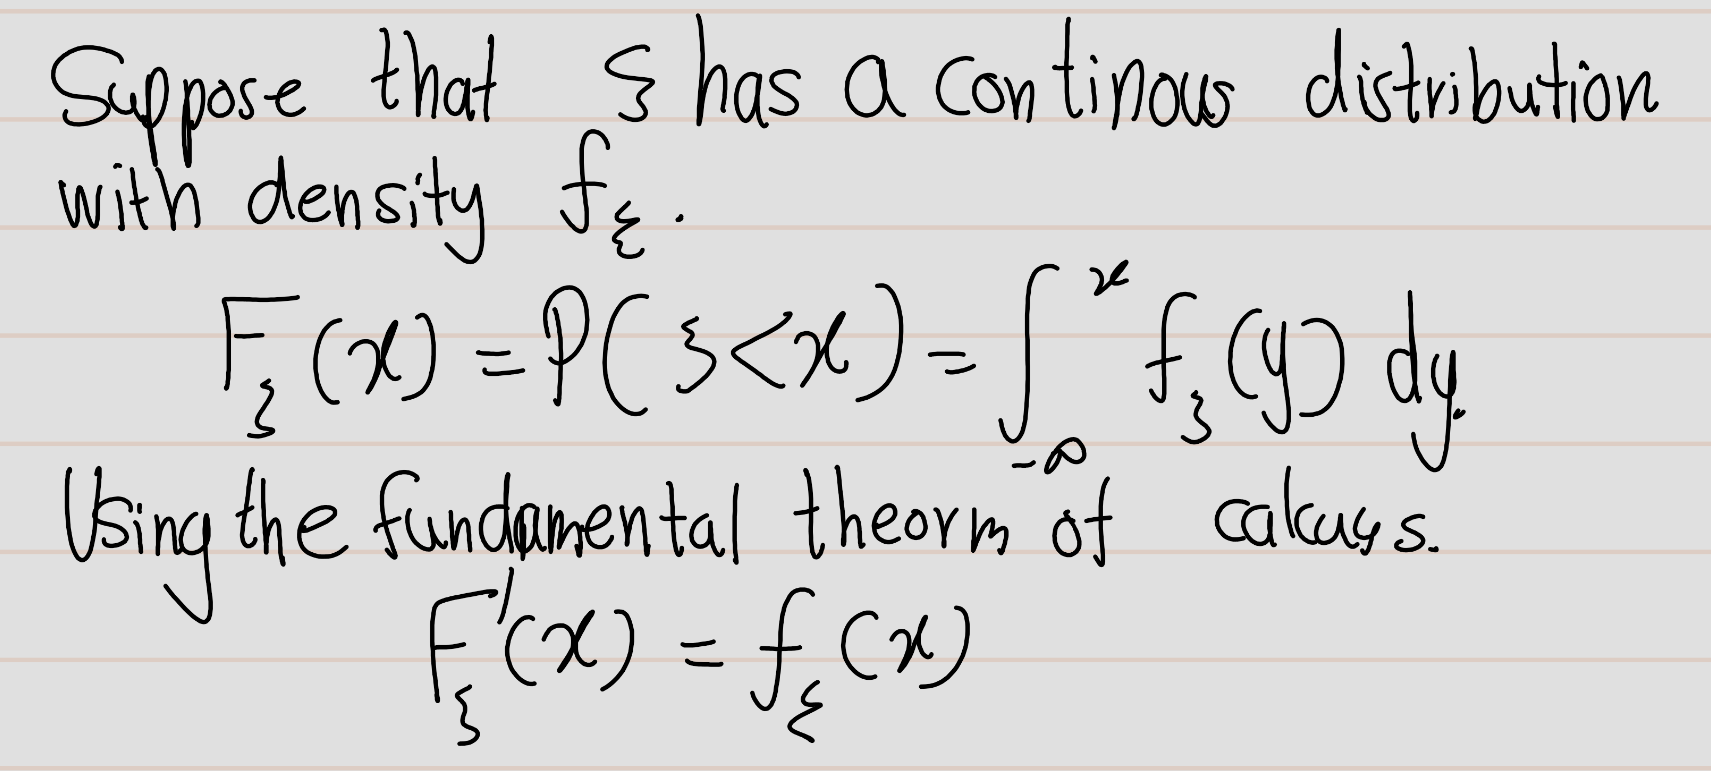
\includegraphics[width=18cm,height=\textheight]{fig/fig ex1.5.png}

Show that if \(\xi\) has discrete distribution with values \(x_1, x_2, . . . ,\) then \(F_\xi\) is
constant on each interval (s, t{]} not containing any of the x\_i's and has jumps of size P \{\xi= x\_i\} at each x\_i·
Hint The increment Fe ( t) - Fe ( s ) is equal to the total mass of the Xi's that belong to the interval {[}s, t).

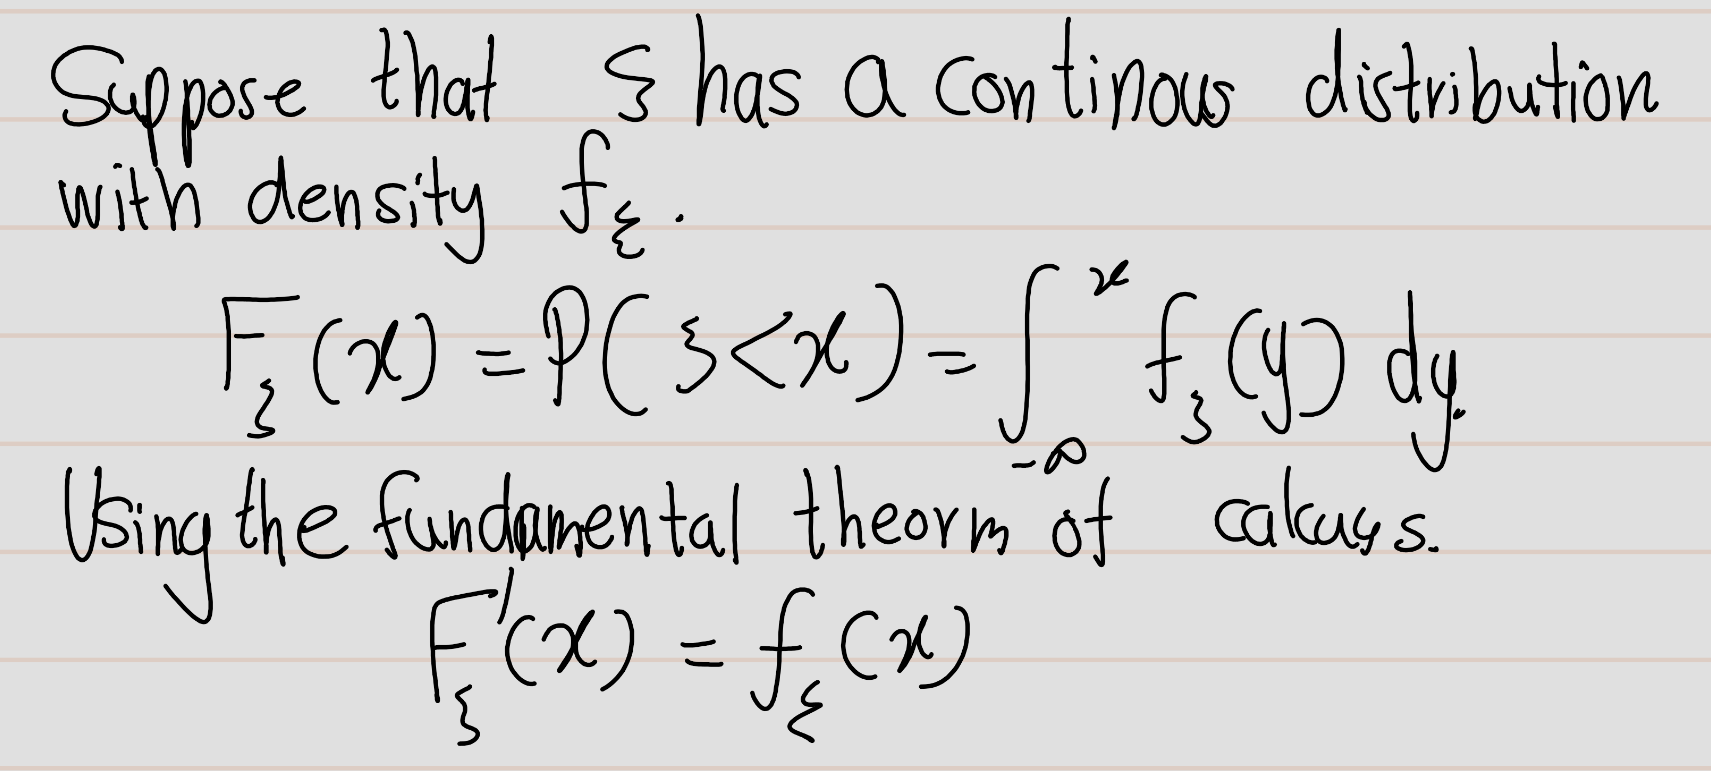
\includegraphics[width=18cm,height=\textheight]{fig/fig ex1.5.png}

\begin{definition}
\protect\hypertarget{def:unnamed-chunk-24}{}\label{def:unnamed-chunk-24}The \textbf{joint distribution} of several random variables \(\xi_1, \ldots, \xi_n\) is a probability measure \(P_{\xi_1, \ldots, \xi_n}\) on \(\mathbb{R}^n\) such that
\[P_{\xi_1, \ldots, \xi_n}(B)=P\left\{\xi_1, \ldots, \xi_n\in B\right\}\]
for any Borel set \(B\) in \(\mathbb{R}^n\). If there is a Borel function \(f_{\xi_1, \ldots, \xi_n} : \mathbb{R}^n \to \mathbb{R}\) such that

\[ P\{(\xi_1, \ldots, \xi_n) \in B\} = \int_B f_{\xi_1, \ldots, \xi_n}(x_1, \ldots, x_n) \, dx_1 \cdots dx_n \]

for any Borel set \(B\) in \(\mathbb{R}^n\), then \(f_{\xi_1, \ldots, \xi_n}\) is called the \textbf{joint density} of \(\xi_1, \ldots, \xi_n\).
\end{definition}

\begin{definition}
\protect\hypertarget{def:unnamed-chunk-25}{}\label{def:unnamed-chunk-25}A random variable \(\xi : \Omega \to \mathbb{R}\) is said to be \textbf{integrable} if

\[ \int_\Omega |\xi| \, dP < \infty. \]

The integral

\[ \mathbb{E}(\xi) = \int_\Omega \xi \, dP \]

exists and is called the expectation of \(\xi\). The family of integrable random variables \(\xi : \Omega \to \mathbb{R}\) will be denoted by \(L^1\) or, in case of possible ambiguity, by \(L^1(\Omega, \mathcal{F}, P)\).
\end{definition}

\begin{example}
\protect\hypertarget{exm:unnamed-chunk-26}{}\label{exm:unnamed-chunk-26}The \textbf{indicator function} \(\mathbf{1}_A\) of a set \(A\) is equal to 1 on \(A\) and 0 on the complement \(\Omega \setminus A\) of \(A\).
i.e.:
\[1_A(a):=\begin{cases} 1 & \text{ if } a \in A  \\0 & \text{ if } a \not\in A\end{cases}  \]

For any event \(A\),
\[\mathbb{E}[1_A]=\int_\Omega 1_A dP=P(A)\]

we say that \(\eta : \Omega \to \mathbb{R}\) is a step function if

\[ \eta = \sum_{i=1}^n \eta_i \mathbf{1}_{A_i}, \]

where \(\eta_1, \ldots, \eta_n\) are real numbers and \(A_1, \ldots, A_n\) are pairwise disjoint events. Then,
\[\mathbb{E}[\eta]=\int_\Omega \eta dP=\sum_{i=1}^n\eta_i \int_\Omega 1_{A_i} dP=\sum_{i=1}^n \eta_i P(A_i)\]
\end{example}

\begin{exercise}
\protect\hypertarget{exr:unnamed-chunk-27}{}\label{exr:unnamed-chunk-27}Show that for any Borel function \(h : \mathbb{R} \to \mathbb{R}\) such that \(h(X)\) is integrable,
\[ \mathbb{E}(h(X)) = \int h(x) \, dP_X(x). \]

\textbf{Hint:} First verify the equality for step functions \(h : \mathbb{R} \to \mathbb{R}\), then for non-negative ones by approximating them by step functions, and finally for arbitrary Borel functions by splitting them into positive and negative parts
\end{exercise}

\textbf{More to go}
\ldots{}

\section{Conditional Probability and Independence}\label{conditional-probability-and-independence}

\begin{definition}
\protect\hypertarget{def:unnamed-chunk-28}{}\label{def:unnamed-chunk-28}For any events \(A, B \in \mathcal{F}\) such that \(P(B) \neq 0\), the conditional probability of \(A\) given \(B\) is defined by
\[P(A \mid B) = \frac{P(A \cap B)}{P(B)}\]
\end{definition}

\begin{exercise}
\protect\hypertarget{exr:unnamed-chunk-29}{}\label{exr:unnamed-chunk-29}Prove the \textbf{total probability formula} for any event \(A \in \mathcal{F}\) and any sequence of pairwise disjoint events \(B_1, B_2, \ldots \in \mathcal{F}\) such that \(B_1 \cup B_2 \cup \cdots = \emptyset\) and \(P(B_n) \neq 0\) for any \(n\).

\textbf{Hint}: \(A = (A \cap B_1) \cup (A \cap B_2) \cup \cdots\)
\end{exercise}

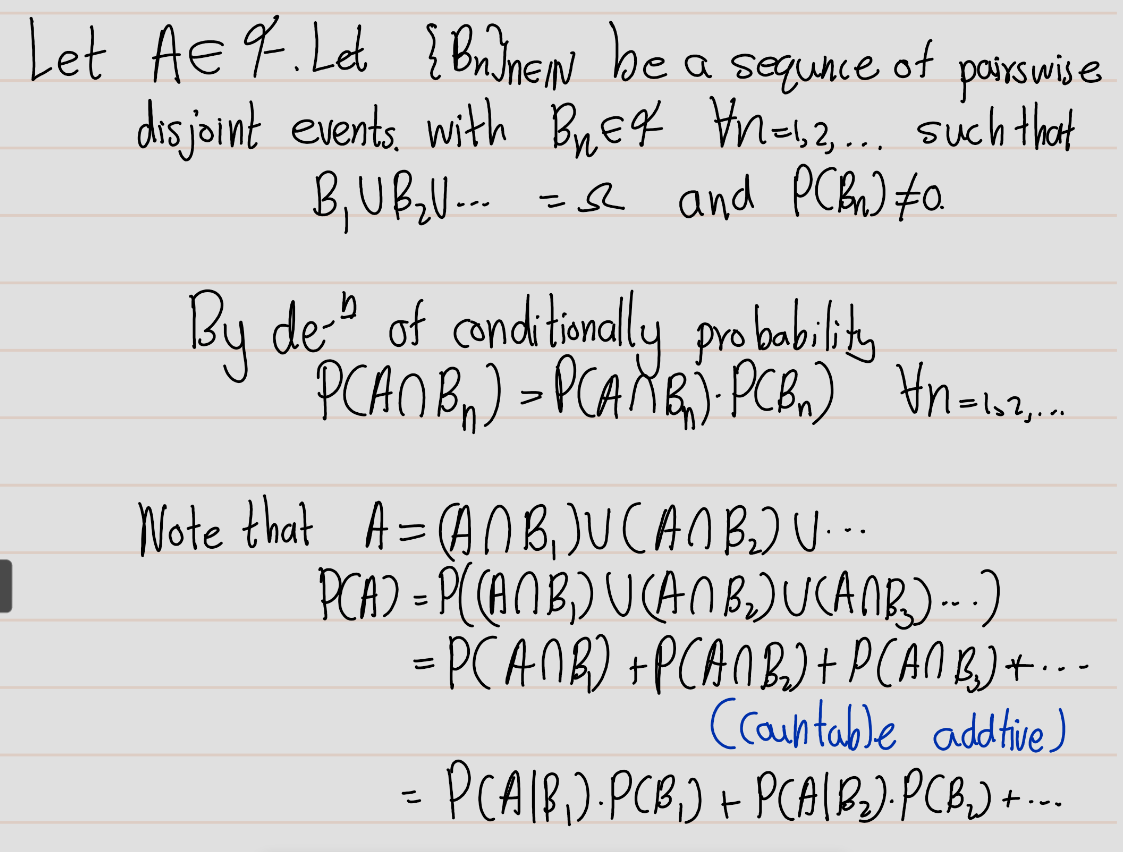
\includegraphics[width=18cm,height=\textheight]{fig/fig ex1.10.png}

\begin{definition}
\protect\hypertarget{def:unnamed-chunk-30}{}\label{def:unnamed-chunk-30}Two events \(A, B \in \mathcal{F}\) are called \textbf{independent} if
\[
P(A \cap B) = P(A)P(B).
\]
In general, we say that \(n\) events \(A_1, \ldots, A_n \in \mathcal{F}\) are \textbf{independent} if for any indices \(1 \leq i_1 < i_2 < \cdots < i_k \leq n\),
\[
P(A_{i_1} \cap A_{i_2} \cap \cdots \cap A_{i_k}) = P(A_{i_1})P(A_{i_2}) \cdots P(A_{i_k}).
\]
\end{definition}

\begin{exercise}
\protect\hypertarget{exr:unnamed-chunk-31}{}\label{exr:unnamed-chunk-31}Let \(P(B) \neq 0\). Show that \(A\) and \(B\) are independent events if and only if
\[
P(A \mid B) = P(A).
\]
\textbf{Hint:} If \(P(B) \neq 0\), then you can divide by it.
\end{exercise}

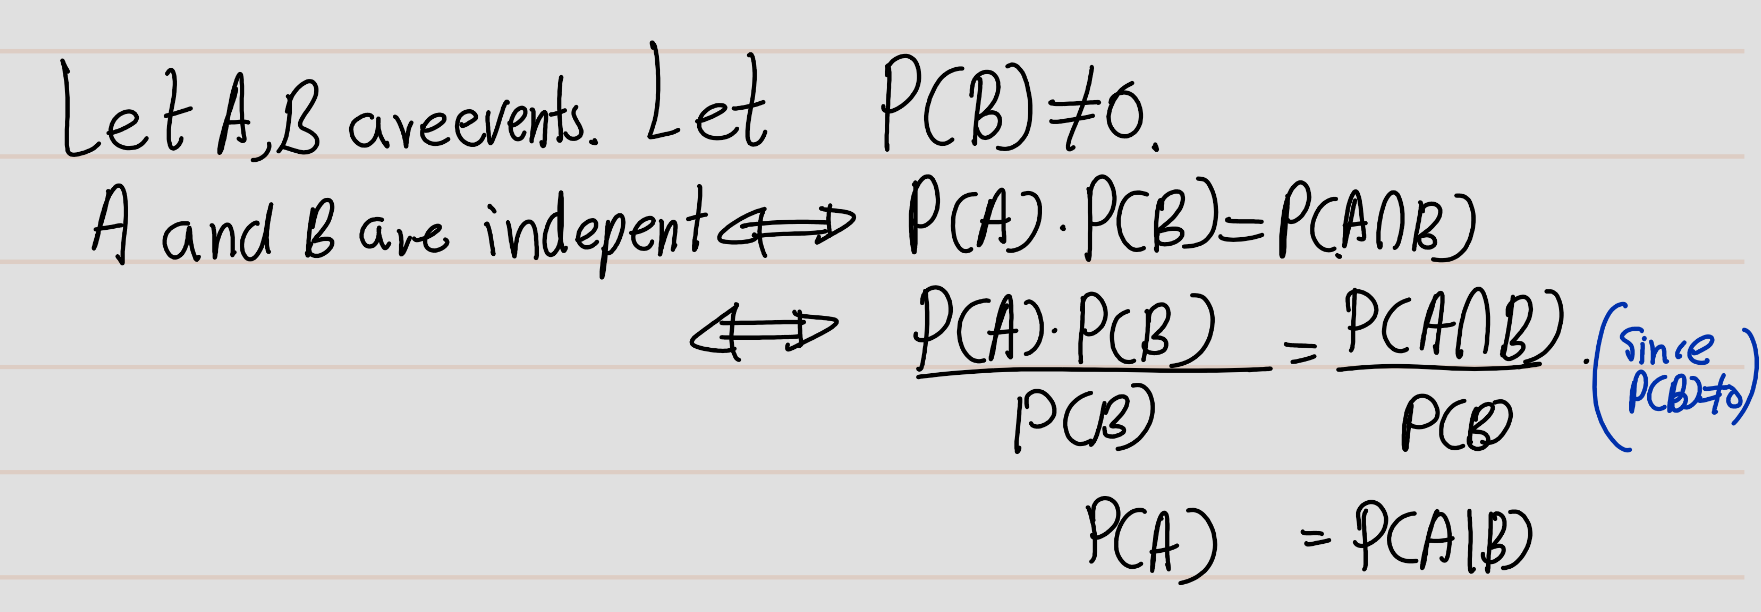
\includegraphics[width=18cm,height=\textheight]{fig/fig ex1.11.png}

\begin{definition}
\protect\hypertarget{def:unnamed-chunk-32}{}\label{def:unnamed-chunk-32}Two random variables \(\xi\) and \(\eta\) are called independent if for any Borel sets \(A, B \in \mathcal{B}(\mathbb{R})\), the two events
\[
\{ \xi \in A \} \text{ and } \{ \eta \in B \}
\]
are independent.

We say that \(n\) random variables \(\xi_1, \ldots, \xi_n\) are independent if for any Borel sets \(B_1, \ldots, B_n \in \mathcal{B}(\mathbb{R})\), the events
\[
\{ \xi_1 \in B_1 \}, \{ \xi_2 \in B_2 \}, \ldots, \{ \xi_n \in B_n \}
\]
are independent.

In general, a (finite or infinite) family of random variables is said to be independent if any finite number of random variables from this family are independent.
\end{definition}

\begin{proposition}
\protect\hypertarget{prp:unnamed-chunk-33}{}\label{prp:unnamed-chunk-33}If two integrable random variables \(\xi, \eta : \Omega \to \mathbb{R}\) are independent, then they are uncorrelated, i.e.,
\[
E(\xi \eta) = E(\xi) E(\eta),
\]
provided that the product \(\xi \eta\) is also integrable.

If \(\xi_1, \ldots, \xi_n : \Omega \to \mathbb{R}\) are independent integrable random variables, then
\[
E(\xi_1 \xi_2 \cdots \xi_n) = E(\xi_1) E(\xi_2) \cdots E(\xi_n),
\]
provided that the product \(\xi_1 \xi_2 \cdots \xi_n\) is also integrable.
\end{proposition}

\begin{definition}
\protect\hypertarget{def:unnamed-chunk-34}{}\label{def:unnamed-chunk-34}Two \(\sigma\)-fields \(\mathcal{G}\) and \(\mathcal{H}\) contained in \(\mathcal{F}\) are called independent if any two events \[ A \in \mathcal{G} \text{ and }   B \in \mathcal{H} \] are independent.

Similarly, any finite number of \(\sigma\)-fields \(\mathcal{G}_1, \ldots, \mathcal{G}_n\) contained in \(\mathcal{F}\) are independent if any \(n\) events \[ A_1 \in \mathcal{G}_1, \ldots, A_n \in \mathcal{G}_n \] are independent.

In general, a (finite or infinite) family of \(\sigma\)-fields is said to be independent if any finite number of them are independent.
\end{definition}

\begin{exercise}
\protect\hypertarget{exr:unnamed-chunk-35}{}\label{exr:unnamed-chunk-35}Show that two random variables \(\xi\) and \(\eta\) are independent if and only if the \(\sigma\)-fields \(\sigma(\xi)\) and \(\sigma(\eta)\) generated by them are independent.

\textbf{Hint:} The events in \(\sigma(\xi)\) and \(\sigma(\eta)\) are of the form \(\{\xi \in A\}\) and \(\{\eta \in B\}\), where \(A\) and \(B\) are Borel sets.
\end{exercise}

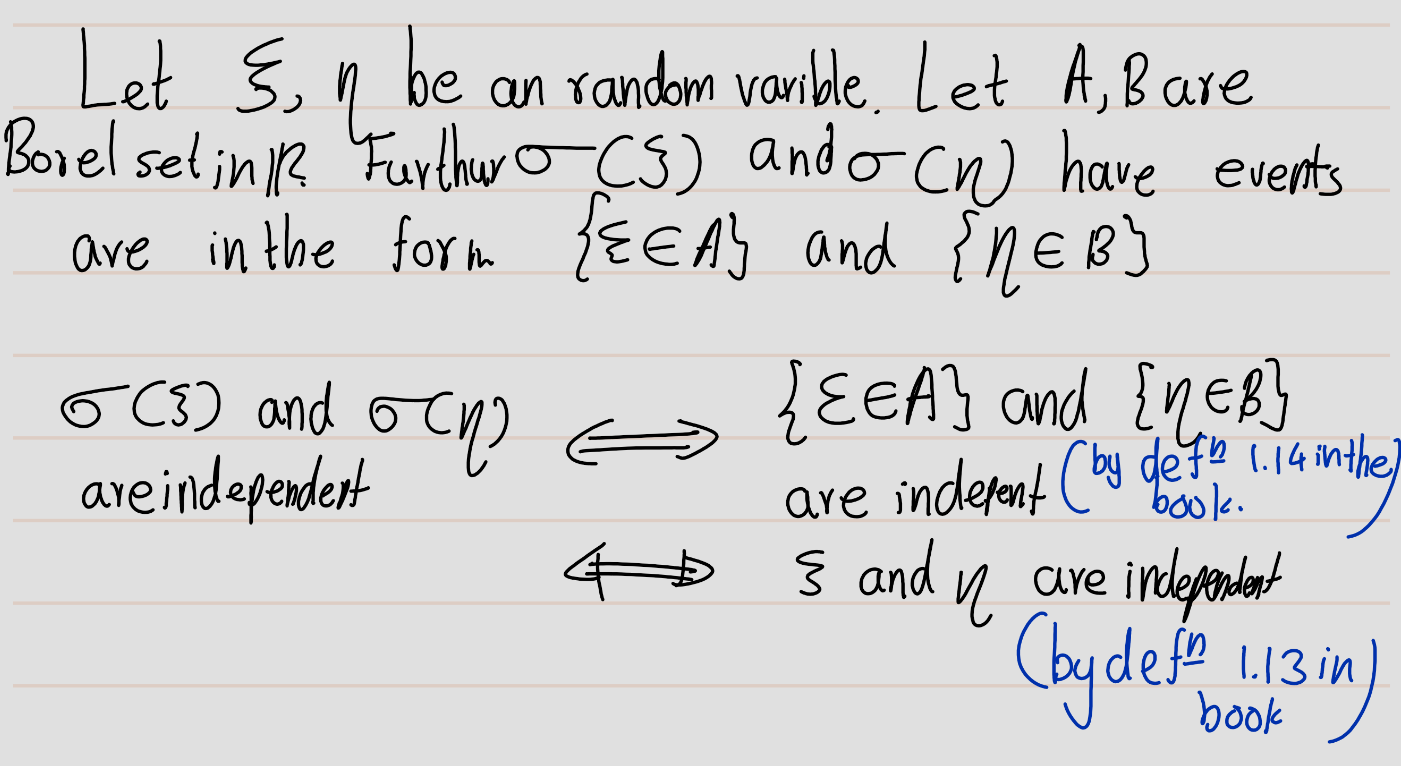
\includegraphics[width=18cm,height=\textheight]{fig/fig ex1.12.png}

Sometimes it is convenient to talk of independence for a combination of random variables and \(\sigma\)-fields.

\begin{definition}
\protect\hypertarget{def:unnamed-chunk-36}{}\label{def:unnamed-chunk-36}We say that a random variable \(\xi\) is independent of a \(\sigma\)-field \(\mathcal{G}\) if the \(\sigma\)-fields \[ \sigma(\xi) \text{ and } \mathcal{G} \] are independent. This can be extended to any (finite or infinite) family consisting of random variables or \(\sigma\)-fields or a combination of them both. Namely, such a family is called independent if for any finite number of random variables \(\xi_1, \ldots, \xi_m\) and \(\sigma\)-fields \(\mathcal{G}_1, \ldots, \mathcal{G}_n\) from this family, the \(\sigma\)-fields
\[\sigma(\xi_1),...,\sigma(\xi_m),\mathcal{G}_1,..,\mathcal{G}_n\]
are independent.
\end{definition}

\chapter{Random Walk to Brownier Motion.}\label{random-walk-to-brownier-motion.}

Slandered approach model stochastic dynamic in discrete time.

Let \(\eta_i\) be an random variable on a conman probability space.
We often \(\Omega,\mathcal{F},P\) assume that i.i.d. This case \(\eta _i\) is called white noise, otherwise coloured noise.
Now we have definite dynamics. It will be given as discreate time dynamical systems recursively by some non linear function.
We define,
\begin{equation}
X_{n+1}=X_n+\phi_{n+1}(X_n,\eta_{n+1}) \quad n=0,1,2,...\label{eq:1}
\end{equation}

where \(\phi_n:\mathbb{R}^d\times \mathbb{R}^d\to \mathbb{R}^d\) are measurable. Further, if \(X_0\) and \(\eta_0\) are all independent then \(X_n\) is called \textbf{Markov Chain}.

Now let \(\eta_i\) be i.i.d and defineda random walk

\begin{align}
S_n&:=\sum_{i=1}^n \eta_i\\
S_{(n+1)}&:=S_n+\eta_{(n+1)}
\end{align}

We can rewrite \eqref{eq:1} as
\[X_{n+1}-X_n=\phi_{n+1}(X_n,S_{n+1}-S_n)\quad n=0,1,...\]

This equation is called \emph{Stochastic difference equations}.

\textbf{AIM}: Develop a continuous time analogous.

\textbf{Question} What to use an contionus time replacement of the random walks?

\begin{definition}
\protect\hypertarget{def:unnamed-chunk-37}{}\label{def:unnamed-chunk-37}Let \(I\) be index set \((I=\mathbb{N} \text{ or } I=\mathbb{R}^+)\). A collection of random varibels \((X_t)_{i\in I}\) on \((\Omega,\mathcal{F},P)\) is called staocastic process.
\end{definition}

We need \(I\) to be a just totally ordered set for convention of time. If it is not an totally ordered set it is not a stochastic process but a random field.

Now we need a notation of a filtration.

\begin{definition}
\protect\hypertarget{def:unnamed-chunk-38}{}\label{def:unnamed-chunk-38}Le \(\mathcal{F}_t\) be non-decreasing sequnce of sub sigma algbers of \(\mathcal{F}\) (i.e.~\(\mathcal{F}_s\subseteq \mathcal{F}_t\) for all \(s\geq t, s,t\in \in I\)), then \((\mathcal{F}_t)_{t\in I}\) is called a filtration.
\end{definition}

Last we need the notation adaptness.

\begin{definition}
\protect\hypertarget{def:unnamed-chunk-39}{}\label{def:unnamed-chunk-39}A stocticstic process \(X_t\) is called adapted to filteration \((\mathcal{F}_t)_t\) if \(X_t\in \mathcal{F}_t\). i.e: \(X_t\) is measurable
\end{definition}

\begin{theorem}[Central Limit Theorem]
\protect\hypertarget{thm:unnamed-chunk-40}{}\label{thm:unnamed-chunk-40}Let \(Y_{n_i}:\Omega \to \mathbb{R}^d\) (be collection of random varibles), \(1\leq i \leq n < \infty\) be identical distributed and square intergable random varaible on \((\Omega,\mathcal{F},P)\) such that \(Y_{n_1},Y_{n_2},...,Y_{n_n}\) are independent for all \(n\in \mathbb{N}\). Then
\[\left(\frac{1}{\sqrt{n}}\sum_{i=1}^n Y_{n_i}-\mathbb{E}[Y_i] \right)
  \xrightarrow{\mathcal{D}} N(0,C) \text{ as } n \to \infty\],
where\(N(0,C)\) is multivarible noremal distribution with covarice matrix \[Y_{k,l}=Cov[Y^{(k)}_{n_i} -Y^{(l)}_{n_i}]\]

and\(\xrightarrow{\mathcal{D}}\) means ``distribution is convergent'' to ```
\end{theorem}

\begin{proof}
Omitted
\end{proof}

We consider the random walk
\[S_n=\sum_{i=1}^n\eta_i\]
with \(\eta_i\in L^2(\Omega,\mathcal{F},P)\) and normalized.(i.e.~\(\mathbb{E}[\eta_i]=0,Var[\eta_i]=1\))

\textbf{Plotting} (Linear Interpolation)
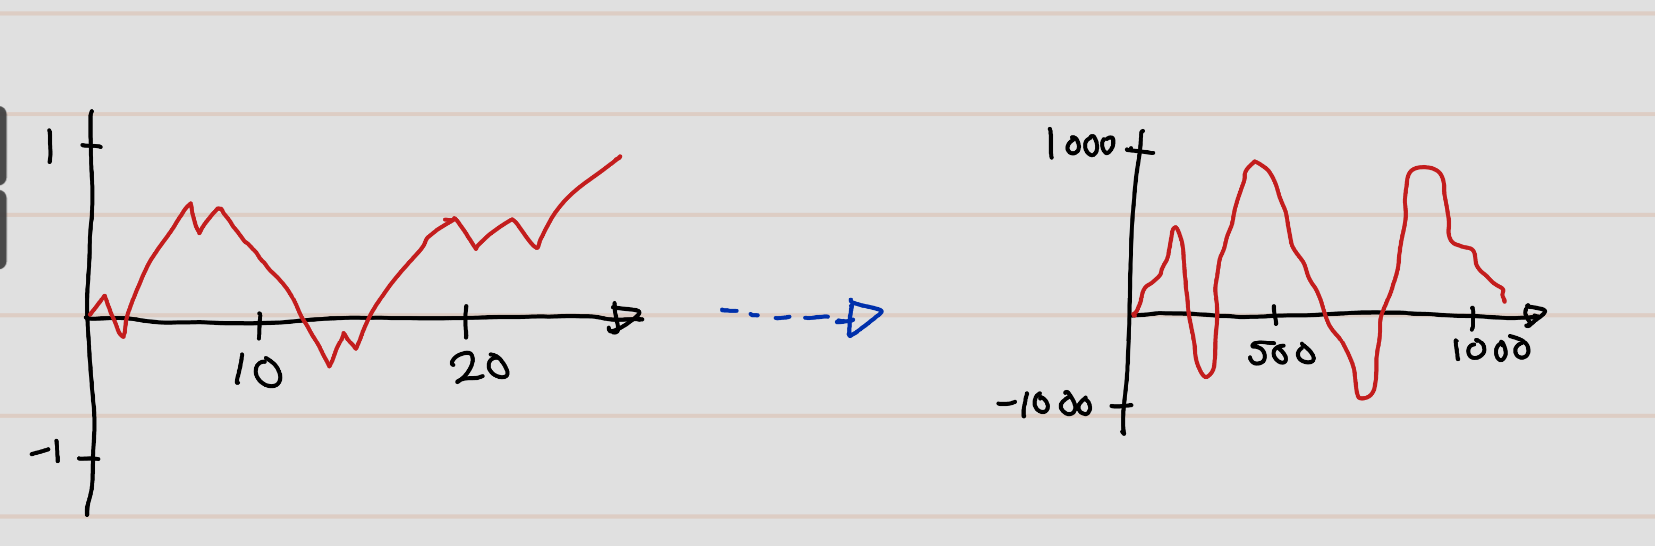
\includegraphics{fig/fig1.png}
This gives an idea about the existance of a scaling limit. Now a question might be rising.

\textbf{Question}: What is right rescaling?

That is we try to define a rescaled random walk \(S^m_t\)(Here superscipt \(m\) is for mesh size),
\((t=0,\frac{1}{m},\frac{2}{m},cdots)\) with step-size \(\frac{1}{m}\)
\[S_{\frac{k}{m}}^{(m)}=c_mS_k\]
Here \(here c_m\) is rescaling constant. It is difficulit to correct \(c_m\), because unless it decay so fast at the end you convert to zero or blow up whole thing and goes to infinity.

For \(t=\frac{k}{m}\) we have
\[Var[S_t^{(m)}]=c^2_m\]

\chapter{Conditional Expectation}\label{conditional-expectation}

\section{Conditioning on an Event}\label{conditioning-on-an-event}

The first and simplest case to consider is that of the conditional expectation
\(\mathbf{E} (\xi|B)\) of a random variable \(\xi\) given an event \(B\).

\begin{definition}
\protect\hypertarget{def:unnamed-chunk-42}{}\label{def:unnamed-chunk-42}For any integrable random variable \(\xi\) and any event \(B \in \mathcal{F}\) such that \(P(B) \neq 0\), the conditional expectation of \(\xi\) given \(B\) is defined by
\[
E(\xi \mid B) = \frac{1}{P(B)} \int_B \xi \, dP.
\]
\end{definition}

\begin{example}
\protect\hypertarget{exm:eg21}{}\label{exm:eg21}Three coins, 10p, 20p, and 50p are tossed. The values of those coins that land heads up are added to work out the total amount \(\xi\). What is the expected total amount \(\xi\) given that two coins have landed heads up?
\end{example}

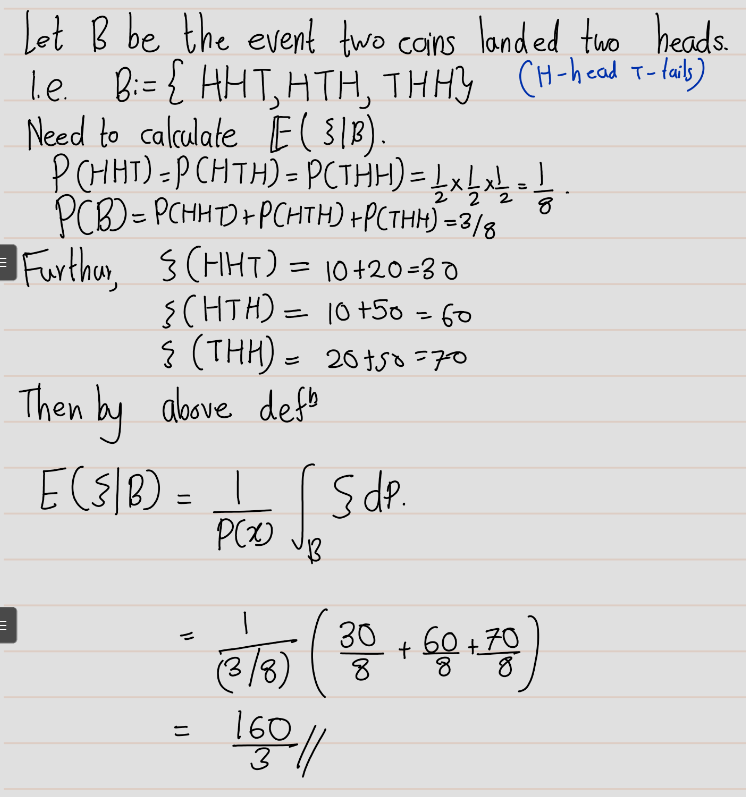
\includegraphics[width=18cm,height=\textheight]{fig/fig eg2.1.png}

\begin{exercise}
\protect\hypertarget{exr:unnamed-chunk-43}{}\label{exr:unnamed-chunk-43}Show that \(E(\xi \mid D) = E(\xi)\).

\textbf{Hint}: The definition of \(E(\xi)\) involves an integral and so does the definition of \(E(\xi \mid D)\). How are these integrals related?
\end{exercise}

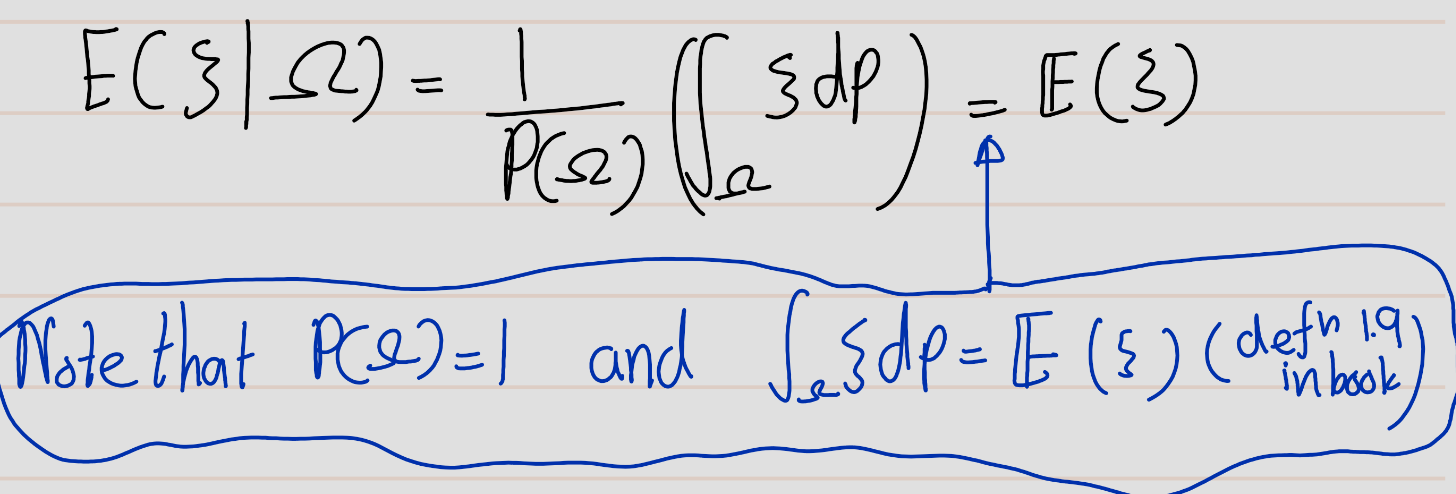
\includegraphics[width=18cm,height=\textheight]{fig/fig ex2.1.png}

\begin{exercise}
\protect\hypertarget{exr:unnamed-chunk-44}{}\label{exr:unnamed-chunk-44}Show that if
\[
\mathbf{1}_A(\omega) = 
\begin{cases} 
1 & \text{for } \omega \in A \\ 
0 & \text{for } \omega \notin A 
\end{cases}
\]
(the indicator function of \(A\)), then
\[
E(\mathbf{1}_A \mid B) = P(A \mid B),
\]
where
\[
P(A \mid B) = \frac{P(A \cap B)}{P(B)}
\]
is the conditional probability of \(A\) given \(B\).

\textbf{Hint}: Write \(\int_B \mathbf{1}_A \, dP\) as \(P(A \cap B)\).
\end{exercise}

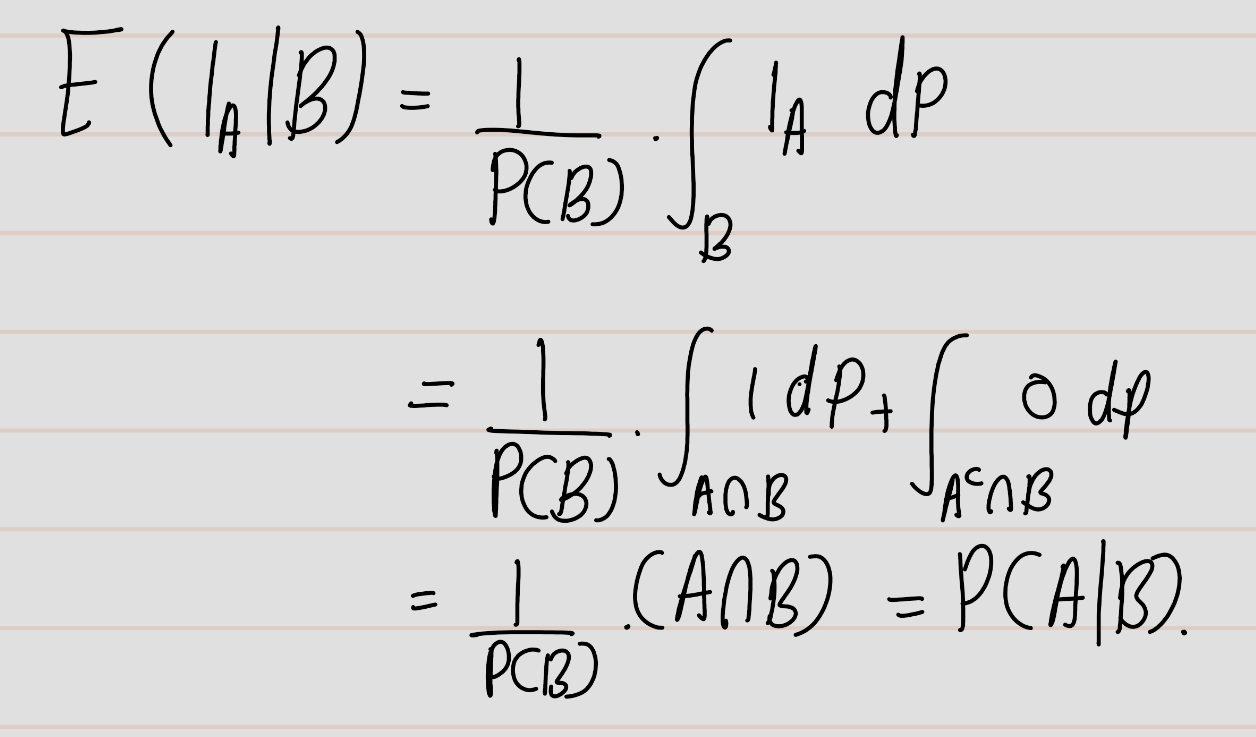
\includegraphics[width=18cm,height=\textheight]{fig/fig ex2.2.png}

\section{Conditioning on a Discrete Random Variable}\label{conditioning-on-a-discrete-random-variable}

The next step towards the general definition of conditional expectation involves conditioning by a discrete random variable \(\eta\) with possible values \(y_1, y_2, \ldots\) such that \(P\{\eta = y_n\} \neq 0\) for each \(n\). Finding out the value of \(\eta\) amounts to finding out which of the events \(\{\eta = y_n\}\) has occurred or not. Conditioning by \(\eta\) should therefore be the same as conditioning by the events \(\{\eta = y_n\}\). Because we do not know in advance which of these events will occur, we need to consider all possibilities, involving a sequence of conditional expectations
\[
E(\xi \mid \{\eta = y_1\}), E(\xi \mid \{\eta = y_2\}), \ldots
\]
A convenient way of doing this is to construct a new discrete random variable constant and equal to \(E(\xi \mid \{\eta = y_n\})\) on each of the sets \(\{\eta = y_n\}\). This leads us to the next definition.

\begin{definition}
\protect\hypertarget{def:unnamed-chunk-45}{}\label{def:unnamed-chunk-45}Let \(\xi\) be an integrable random variable and let \(\eta\) be a discrete random variable as above. Then the conditional expectation of \(\xi\) given \(\eta\) is defined to be a random variable \(E(\xi \mid \eta)\) such that
\[
E(\xi \mid \eta)(\omega) = E(\xi \mid \{\eta = y_n\}) \text{ if } \eta(\omega) = y_n
\]
for any \(n = 1, 2, \ldots\).
\end{definition}

\begin{example}
\protect\hypertarget{exm:unnamed-chunk-46}{}\label{exm:unnamed-chunk-46}Three coins, 10p, 20p, and 50p are tossed as in Example \ref{exm:eg21}. What is the conditional expectation \(E(\xi \mid \eta)\) of the total amount \(\xi\) shown by the three coins given the total amount \(\eta\) shown by the 10p and 20p coins only?
\end{example}

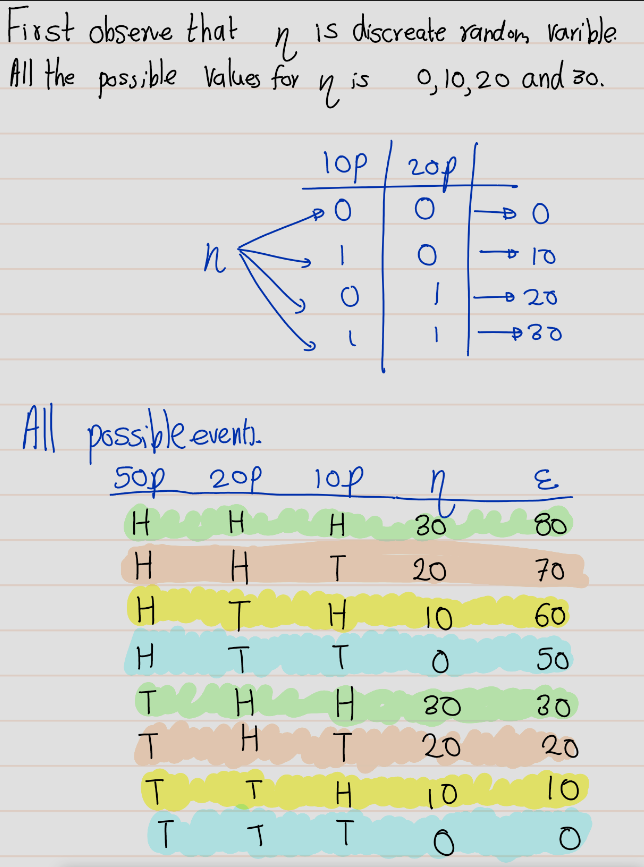
\includegraphics[width=18cm,height=\textheight]{fig/fig eg2.2-1.png}
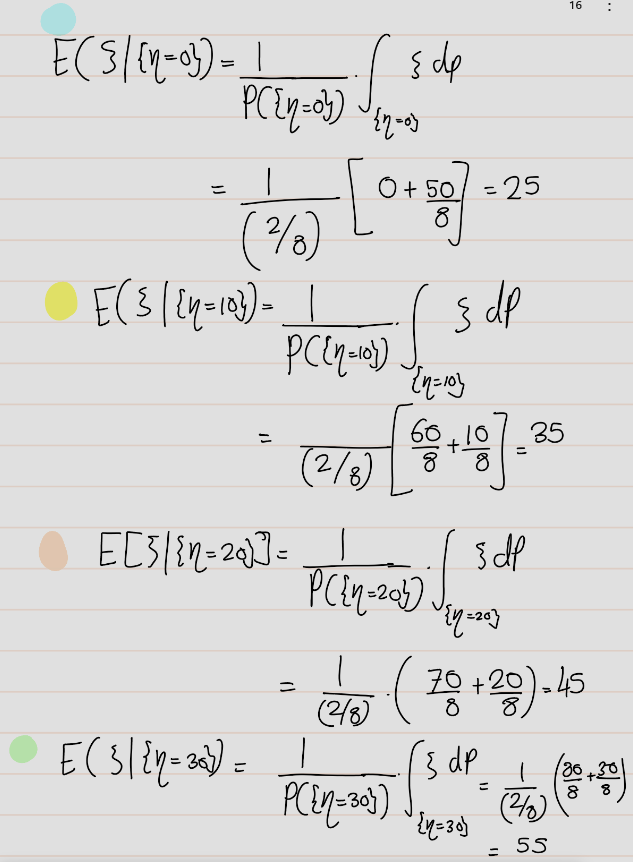
\includegraphics[width=18cm,height=\textheight]{fig/fig eg2.2-2.png}
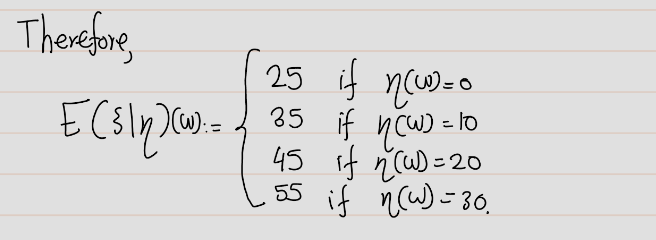
\includegraphics[width=18cm,height=\textheight]{fig/fig eg2.2-3.png}

\chapter{Les}\label{les}

\section{Integrals}\label{integrals}

First we review the definitions of the Riemann integral in calculus and the Riemann--Stieltjes integral in advanced calculus.

\subsection{Riemann Integral}\label{riemann-integral}

Let \(f\) be an bounded function defined on a finite closed interval \([a, b]\). Then \(f\) is called \emph{Riemann integrable} if the following limit exists.
\begin{equation}
x
\end{equation}

\section{Random Walks}\label{random-walks}

Consider a random walk starting at 0 with jumps \(h\) and \(-h\) equally likely at times \(\delta, 2\delta,...\), where \(h,\delta>0\) . More precisely, let \(\{X_n\}_{n=1}^\infty\) be a sequence of independent and identically distributed random variables with
\[P(X_j = h) = P(X_j = −h) = \frac{1}{2}\]

Let \(Y_{\delta,h}(0) =0\)
\[Y_{\delta,h}(n\delta) = X_1 + X_2 + \ldots + X_n\]
For \(t > 0\) define \(Y_{\delta,h}(t)\) by linearization:
(i.e: For \(n\delta < t < (n + 1)\delta\), define
\[Y_{\delta,h}(t) = \frac{(n + 1)\delta - t}{\delta} Y_{\delta,h}(n\delta) + \frac{t - n\delta}{\delta} Y_{\delta,h}((n + 1)\delta).\]

  \bibliography{book.bib,packages.bib}

\end{document}
